\section{Experiments and Results}

\begin{frame}
	\frametitle{\secname\ Overview}
	\tableofcontents[currentsection]
\end{frame}

\subsection{3-Clique merge with insertion}
\begin{frame}
	\frametitle{Method}
	Planetoid/Cora dataset:

	\begin{itemize}
		\item Node classification problem
		\item 2708 nodes (7 classes)
		\item 10556 edges (undirected)
		\item 1433 features per node (number of occurrences of words)
		\item 5\% training node label rate
		\item 100 runs with 300 epochs
	\end{itemize}
\end{frame}

\begin{frame}{\subsecname\ Description}
	\begin{enumerate}
		\item Find all 3-cliques from a graph and save them in a list
		\item Sort them according to sum of pairwise distances
		\item Repeat the following steps until there are any nodes in a list:
		      \begin{enumerate}
			      \item Take the `top' 3-clique
			      \item Save \emph{all} edges coming in/out of the clique
			      \item Compute a `generic feature vector' by taking average of their feature vectors
			      \item Delete them from the graph
			      \item Create a new `merged' node with a generic feature vector and all saved edges
			      \item Filter out the deleted nodes from list of 3-cliques
		      \end{enumerate}
	\end{enumerate}
\end{frame}

\begin{frame}[allowframebreaks]
	\frametitle{3-clique Merge Example}

	The following figures show exactly how a 3-clique is merged: the resulting feature vector is the average of the feature vectors of initial nodes: $\frac{1}{3} \cdot \left( (1, 4, 5) + (2, 7, 1) + (0, 1, 6) \right) = \frac{1}{3} \cdot (3, 12, 12) = (1, 4, 4)$

	\begin{figure}[h]
		\begin{minipage}{.7\textwidth}
			\centering
			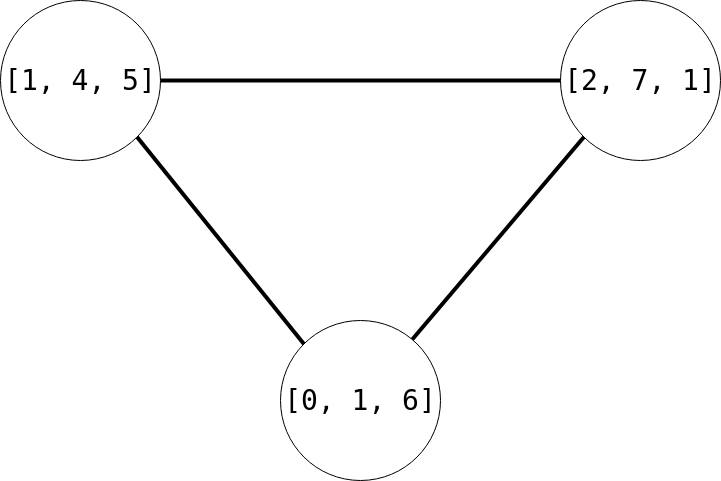
\includegraphics[width=0.8\linewidth]{3clique_before_merge_example}
		\end{minipage}%
		\begin{minipage}{.3\textwidth}
			\centering
			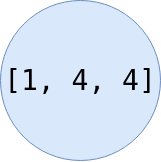
\includegraphics[width=0.6\linewidth]{3clique_merged_example}
		\end{minipage}
	\end{figure}

	\framebreak

	\begin{figure}[h]
		\begin{multicols}{2}
			\centering
			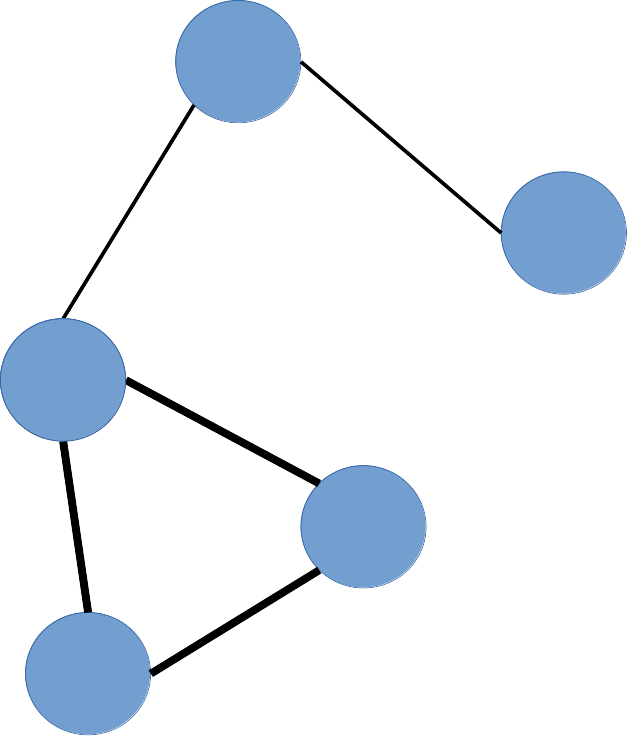
\includegraphics[width=0.4\textwidth]{simplex_1.png}
			\caption{A part of some graph}\label{fig:clique_merged}

			\centering
			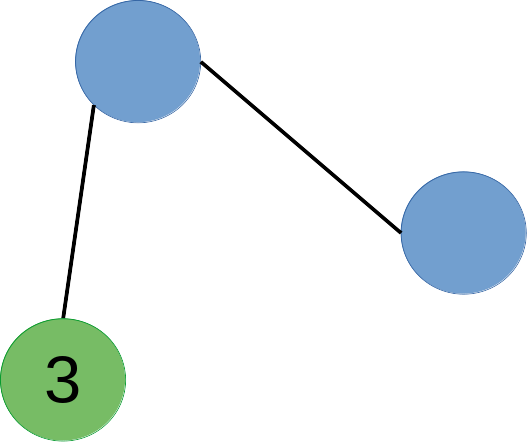
\includegraphics[width=0.4\textwidth]{simplex_2.png}
			\caption{Three nodes from the left image united in 3-simplex having properties of the initial vertices}
		\end{multicols}
	\end{figure}
\end{frame}

\begin{frame}[allowframebreaks, c]
	\frametitle{Results}

	\centering
	\begin{tabular}{ |c|c|c|c| }
		\hline
		Feature       & Before & After  & Delta   \\
		\hline
		Node num      & 2708   & 2120   & 21.71\% \\
		Edge num      & 10556  & 4568   & 56.73\% \\
		Learning time & 4.171s & 2.939s & 29.5\%  \\
		Accuracy      & 0.803  & 0.746  & 7\%     \\
		\hline
	\end{tabular}

	\framebreak

	Accuracies graph:
	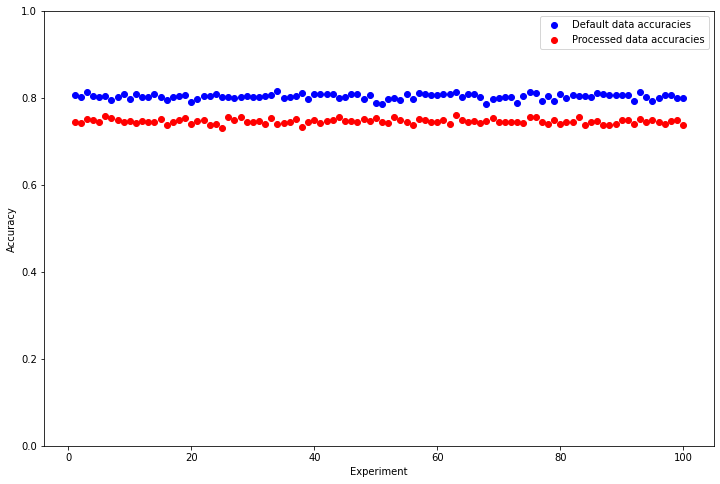
\includegraphics[height=0.85\textheight]{3clique_accuracy.png}
\end{frame}

\subsection{Infinite 3-clique merge with insertion}

\begin{frame}{\subsecname\ Description}
	In this experiment, the methodology and the algorithm are similar to the `finite 3-clique merge'.
	The only difference is that we \emph{allow} merged nodes to participate in merge process again.
\end{frame}

\subsubsection*{Results and interpretation}
\begin{frame}[allowframebreaks]
	\frametitle{Results}
	The proposed method allowed us to remove the majority of information from a graph.

	\centering
	\begin{tabular}{ |c|c|c|c| }
		\hline
		Feature       & Before & After  & Delta   \\
		\hline
		Node num      & 2708   & 1080   & 60.12\% \\
		Edge num      & 10556  & 656    & 93.79\% \\
		Learning time & 2.537s & 1.059s & 58\%    \\
		Accuracy      & 0.809  & 0.517  & 36\%    \\
		\hline
	\end{tabular}

	\framebreak

	\begin{figure}[h]
		\centering
		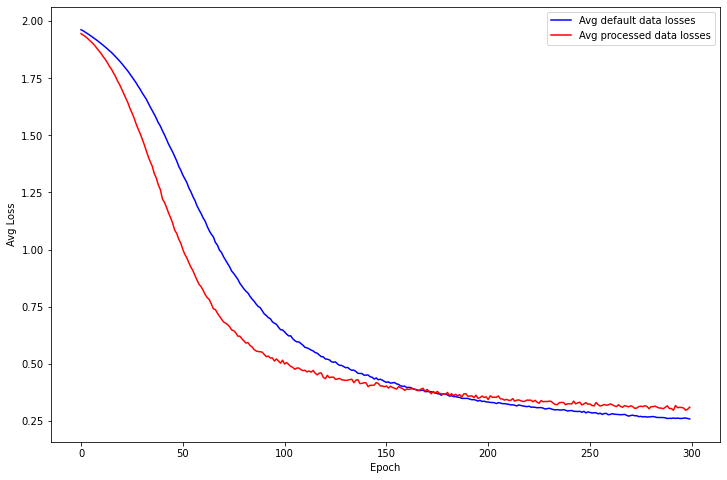
\includegraphics[height=0.85\textheight]{3clique_inf_loss}
		\caption{Average loss for `default' and processed data}
	\end{figure}
\end{frame}

\subsection{Prospects}
\begin{frame}{\subsecname}
	In future we want to focus on topological aspect of the transformation presented in the paper.
	In particular, we are interested in `infinite merge', where `merged nodes' can be merged again.
	We also want to see how the transformation presented can be used in other tasks, for example, in graph classification.
\end{frame}
